\section{Wybrane aspekty realizacji}
\label{sec:wybrane-aspekty-realizacji}

% \emph{Przyjęte założenia, struktura i zasada działania systemu,
  % wykorzystane rozwiązania technologiczne wraz z krótkim uzasadnieniem
  % ich wyboru.}

Głównym celem produktu końcowego jest udostępnienie użytkownikowi funkcjonalności szyfrowania i deszyfrowania plików. Celem pobocznym przedsięwzięcia projektowego jest eksploracja zagadnienia wykorzystania układów logiki programowalnej FPGA do rozwiązywania problemów dziedziny kryptografii na przykładzie algorytmu AES.

\subsection {Struktura i zasada działania systemu}
Projekt jest zbudowany w oparciu o architekturę klient-serwer (rys. \ref{fig:system-architecture}). Rolę serwera pełni płytka Terasic DE1-SOC, a klientem jest komputer PC. Komunikacja odbywa się przez kabel USB, przez który tunelowany jest sygnał UART.

\begin{figure}[!h]
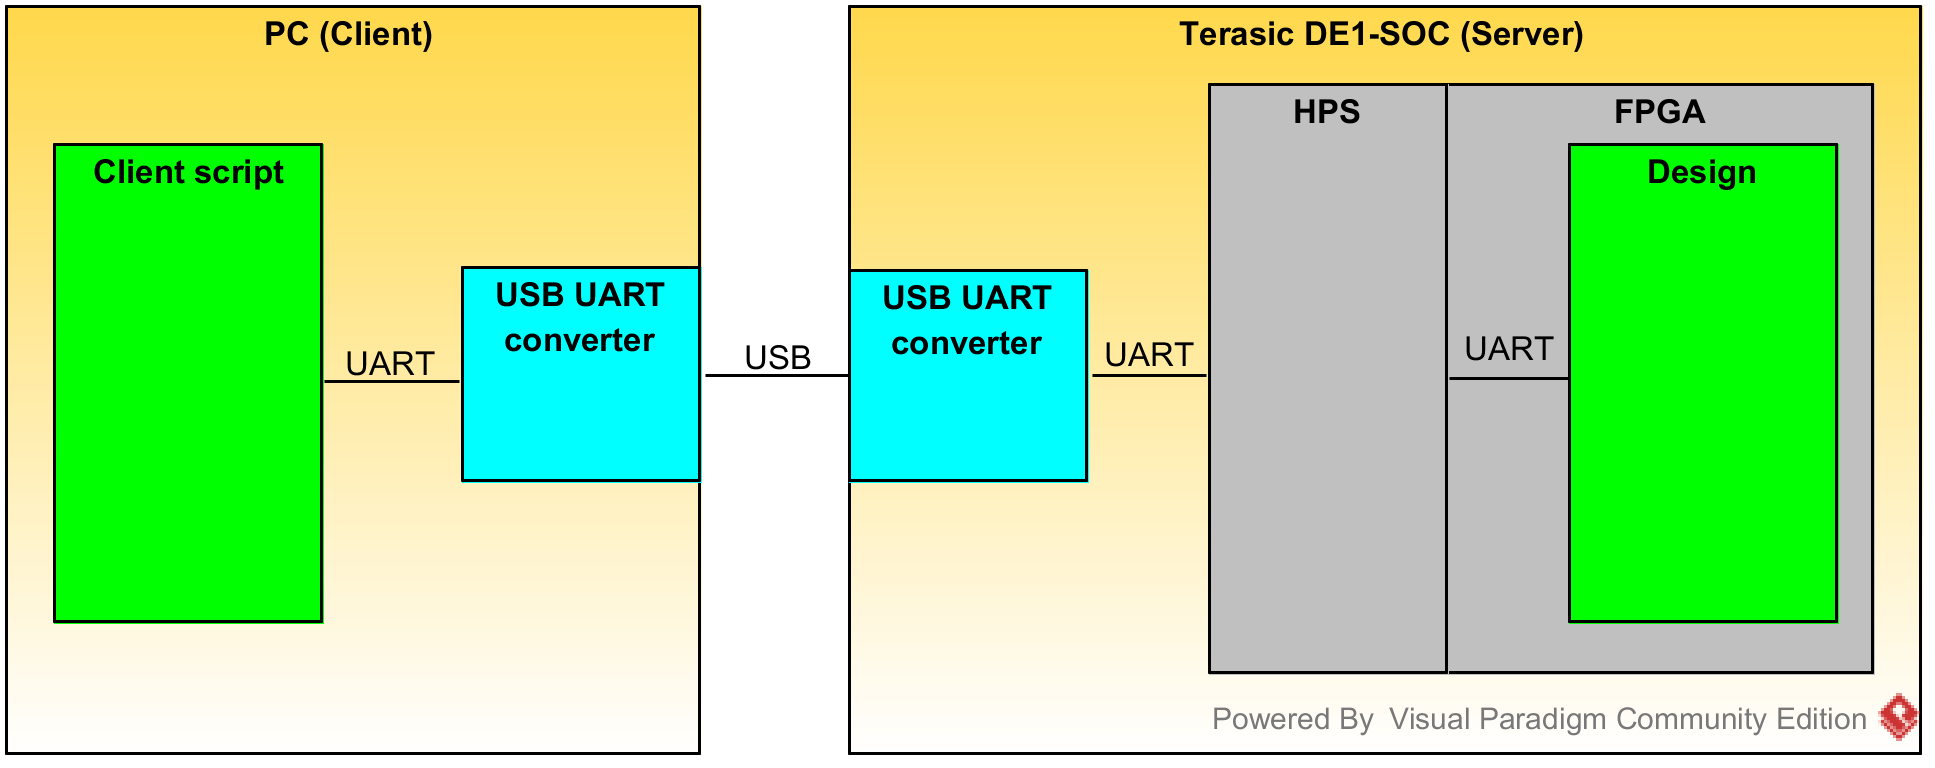
\includegraphics{pictures/system-architecture.png}
\caption{Części składowe systemu}
\label{fig:system-architecture}
\end{figure}

Serwer (płytka Terasic DE1-SOC) wyposażony jest w układ FPGA, którego zadaniami są:
\begin{itemize}
\item obsługa protokołu komunikacji UART oraz obsługa błędów
\item odbieranie bloków danych od klienta oraz odsyłanie ich w przetworzonej formie
\item szyfrowanie i deszyfrowanie odbieranych bloków algorytmem AES w trybie łączenia bloków CBC
\end{itemize}

Klientem jest komputer PC z systemem operacyjnym Ubuntu. Programem udostępniającym użytkownikowi funkcjonalność szyfrowania i deszyfrowania plików jest skrypt, który:
\begin{itemize}
\item odczytuje z dysku pliki do zaszyfrowania
\item dzieli je na bloki, które wysyła do serwera w celu zaszyfrowania lub odszyfrowania
\item odbiera przetworzone bloki danych oraz zapisuje je na dysku 
\end{itemize}

Komunikacja między klientem a serwerem odbywa się przez kabel USB, którym tunelowany jest sygnał UART. Końcówką tunelu po stronie serwera jest konwerter UART-USB firmy FTDI. Po stronie klienta tunel obsługiwany jest przez wbudowany w system operacyjny sterownik, który umożliwia realizację komunikacji w sposób analogiczny do zwykłego portu szeregowego. Wykorzystany układ Altera Cyclone V zawiera zintegrowany procesor HPS do którego podłączone są sygnały UART, w wyniku czego muszą one przechodzić przez piny HPS. Procesor nie wykonuje żadnych obliczeń ani nie modyfikuje sygnałów UART.

\subsection{Wykorzystane rozwiązania technologiczne}
Projekt jest realizowany na platformie FPGA. Układy FPGA, w przeciwieństwie do procesorów CPU, nie mają z góry ustalonej struktury -- schemat układu jest programowalny. Daje to możliwość projektowania wysoce wyspecjalizowanych układów, które będą miały strukturę zoptymalizowaną pod kątem wykonywania konkretnego zadania. Takie podejście jest znacząco różne od procesorów CPU, które są w stanie wykonywać jedynie z góry określone zestawy instrukcji ogólnego przeznaczenia. Stanowi do duże ograniczenie procesorów oraz powoduje, że dobrze zaprojektowane i zoptymalizowane układy zrealizowane na FPGA mogą być znacząco bardziej wydajne niż programy będące ich odpowiednikami wykonywane na CPU.

\begin{figure}[!h]
\centering
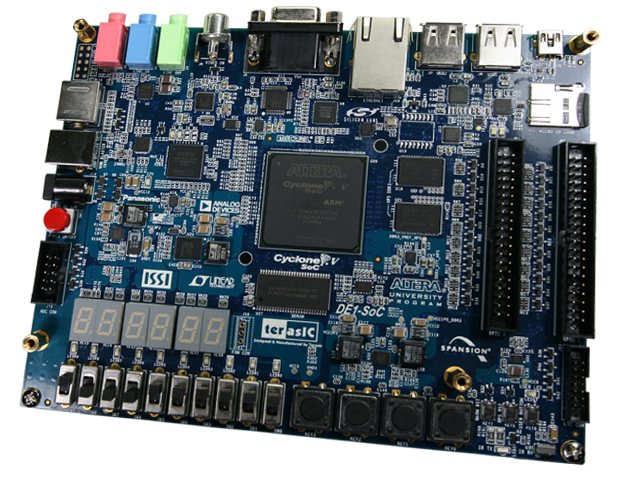
\includegraphics[width=\textwidth]{pictures/fpga-board.jpg}
\caption{Płytka Terasic DE1-SOC \cite{plytka}}
\label{fig:fpga-board}
\end{figure}

Płytką FPGA użytą do realizacji projektu jest Terasic DE1-SoC (rys. \ref{fig:fpga-board}). Została ona wybrana, ponieważ:
\begin{itemize}
\item Układ FPGA, w który jest wyposażona ma dużą liczbę jednostek logicznych oraz zintegrowany procesor ARM. Pozwoli to na zrealizowanie wymagania dotyczącego automatycznego programowania układu przy starcie płytki. Obecność zintegrowanego procesora była pożądana przy wyborze również ze względu na fakt, że nabyty sprzęt może być w przyszłości użyty do realizacji innych projektów, które mogą wymagać takiej funkcjonalności.
\item Płytka jest wyposażona w konwerter USB-UART, co eliminuje konieczność korzystania z oddzielnego produktu realizującego tą funkcjonalność.
\item Układ FPGA znajdujący się na płytce jest firmy Altera, co miało znaczenie ze względu na fakt, że zespół projektowy miał doświadczenie z pracą ze środowiskiem developerskim wspierającym tą technologię (Quartus).
\end{itemize}

Do komunikacji między komputerem a płytką FPGA wykorzystywany jest protokół UART ze względu ja jego prostotę. Podjęto taką decyzję ponieważ zespół projektowy tylko jednoosobowy i głównym celem projektu była implementacja algorytmu AES. Wykorzystanie bardziej złożonego protokołu komunikacji (np. USB lub Ethernet) pozwoliłoby na osiągnięcie większej szybkości transmisji, lecz wiązałoby się z koniecznością poświęcenia większej ilości czasu na implementację jego obsługi. Dostępne zasoby ludzkie nie pozwalały na zrealizowanie takiego zadania w dostępnym czasie.

Środowiskiem programistycznym, które posłużyło do stworzenia projektu FPGA jest Quartus. Wybór ten był podyktowany faktem, że płytka Terasic DE1-SOC jest wyposażona w układ FPGA firmy Altera. Wykorzystanym do napisania projektu FPGA językiem programowania był VHDL, ponieważ zapewnia silną kontrolę typów podczas kompilacji. Program komputerowy zostałZ napisany w języku Python, gdyż pozwala on na wygodną obsługę odczytu i zapisu plików oraz sterowanie transmisją UART. Więcej szczegółów dotyczących wykorzystanych narzędzi developerskich znajduje się w dokumentacji technicznej.


\newpage